\section{Proposed Method}

The methodology in this to first address the \gls{MVP}, and state the
specifications for a \gls{MVP}, see Section \ref{sec:mvs}. From there, features
will then be added
according to a feature list, see Section \ref{sec:features}.

\subsection{Minimum viable solution}\label{sec:mvs}

Initially, the project to aims to address the mapping phase, and if time allows
implement a localization module as well. Since the idea is that the data will
be ``crowd sourced'' the sensors cannot be expected to be high cost, therefore
\gls{LIDAR} measurements are not initially considered. The types of sensor that
first will be investigated are radio measurements, \gls{GNSS}, inertial
navigation, and camera sensors.

Due to the separation of landmarks in radio and camera measurements, these two
systems can provide an independent estimate of the dynamical states, $x_{1:T}$
and the separate landmarks $m_{r,1:T}$ for radio and $m_{v,1:T}$ for the
camera.

\subsection{Sensor Fusion}

The sensor fusion will be performed using a combination of particle
filters and the \gls{EM} algorithm
\cite{DBLP:journals/automatica/SchonWN11}. Particle filters
\cite{210672} has been used to compute unbiased estimates of the
states $x_{t}$  of non-linear and non-Gaussian state space models. In
this algorithm several hypotheses, or particles, are propagated and
compared to the observed measurements. The hypotheses that eventually
are considered unlikely are discarded, the likely ones are
propagated. The main advantage of the particle filter is that the
different sensor modalities only have to supple a measurement function
of the type:
$$
y_k = h(x_k, m) + e_k,
$$
which depends on the current dynamical state of the vehicle, $x_t$ and
the positions of the landmark $m$. It is assumed here that the sensor
noise is additive, but it does not have to be.

However, the particle filters suffers from the curse of
dimensionality, i.e., if the state vector is large $x_t$ the
computational burden becomes in-feasible \cite{1453762}. To include
thousands of landmarks $m$ can thus be difficult. And the knowledge
that the landmarks are static in time is hard to incorporate into the
particle filter solution.

Thus, to approach the problem of estimation of landmark positions, the
\gls{EM}-algorithm \cite{Dempster77maximumlikelihood} will be employed
as well. The\gls{EM}-algorithm is an iterative procedure for computing
the \gls{ML} estimator when only a subset of the data is available. It
consists of two steps: one expectation step and one maximization
step. For purpose of this project, the particle filter will be used to compute
unbiased estimates of the log-likelihood of the measurements for a
given value of the landmark positions. Then in the maximization step,
new landmark positions will be computed.



\subsection{Motion model}

As a motion model for dynamics of the vehicle, we will use the bicycle model
adapted for a
car.
The parameters are shown in figure \ref{fig:motion_model}. The state space
model is defined as

\begin{equation}
 \begin{array}[b]{r}
  \dot{x}  = v \cos \theta \\
  \dot{y}  = v \sin \theta \\
  \dot{\theta}  = \frac{v}{L} \tan{\phi}
 \end{array}
\end{equation}

where $v$ is speed of the car and $\phi$ is the steering angle.
These can be observed using an \gls{IMU} and/or estimates from the onboard car
sensors. This provides a model for $f_k$ in Equations \eqref{eq:slam_problem}.

\begin{figure}
\centering
\label{fig:motion_model}
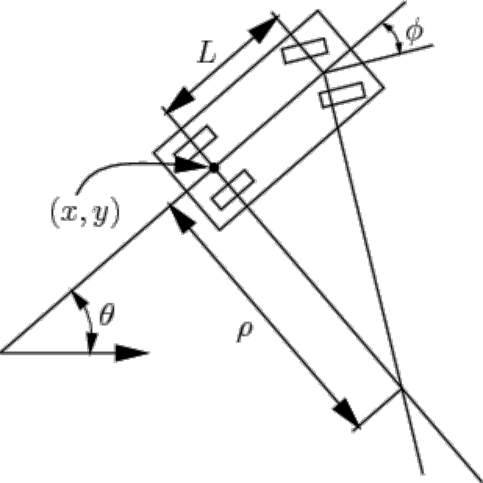
\includegraphics[width=0.3\textwidth]{figures/bicycle_model.pdf}
\caption{Bicycle motion model adapted for car}
\end{figure}


\subsection{Radio Measurements}\label{sec:radio_measurements}


The radio based localization could be summarized as three steps:

\begin{itemize}
\item Radio channel data collection. There are two options:
  \begin{itemize}
  \item To use channel sounder and antenna arrays (with 32 antenna
    elements) on both base station and user sides to collect channel
    information with respect to angles and distances.
  \item To use an \gls{USRP} with \gls{LTE} framework and switching antenna array to
  receive commercial \gls{LTE} signals from base stations.
\end{itemize}
\item  High spatial sampling rate of the radio channel is required, typically a few samples per wavelength movement.
\item Radio channel parameter estimation. This could be done using the \gls{EKF} or the
\gls{SAGE} based estimator
to extract geometrical information of the environment, i.e., propagation path
parameters:
\begin{itemize}
\item the azimuth/elevation angle of arrival,
\item propagation
distance,
\item etc.
\end{itemize}
\end{itemize}

The measurements of the radio channel could be modelled as the
combination of the specular components $ \mathbf{h}_{sp} $, \gls{DMC}
$ \mathbf{h}_{dmc} $ and measurement noise $
\mathbf{h}_n $, yielding:
\begin{equation}
\mathbf{y}_k = \mathbf{h}_{sp} + \mathbf{h}_{dmc} + \mathbf{h}_n.
\label{eq:channelmodel}
\end{equation}
Radio based SLAM relies on the geometrical information from $
\mathbf{h}_{sp} $, which is characterized as a superposition of
specular \gls{MPC}s. $ \mathbf{h}_{dmc} $ and $ \mathbf{h}_n $
constitute measurement impairments for our purpose, which is further
modelled as the covariance matrix. $ \mathbf{h}_{sp} $ could be
further formulated as:

\begin{equation}
\mathbf{h}_{sp} = \textbf{s}(\mathbf{\boldsymbol{\mu}_k}, \mathbf{\boldsymbol{\gamma}}_k).
\label{eq:channelmodel}
\end{equation}
\begin{equation}
\mathbf{\boldsymbol{\mu}} = [\mathbf{\boldsymbol{d}}^\text{T} \quad  \mathbf{\boldsymbol{\varphi}}^\text{T}_\text{Tx} \quad  \mathbf{\boldsymbol{\theta}}^\text{T}_\text{Tx} \quad \mathbf{\boldsymbol{\varphi}}^\text{T}_\text{Rx} \quad  \mathbf{\boldsymbol{\theta}}^\text{T}_\text{Rx}],
\end{equation}
where $ \mathbf{\boldsymbol{d}} $ is the propagation distance of each
\gls{MPC} from the base station to the the vehicle. $
\mathbf{\boldsymbol{\varphi}} $ and $ \mathbf{\boldsymbol{\theta}} $
represent the azimuth and elevation \gls{AOA} in the 3D space on both
sides. These geometrical information related to the environment will
be further used for the localization of the vehicle and mapping.


The radio channel measurement will be performed locally in Lund. For
sensor fusion in the late phase of this project, the measurement with
different sensors will be performed simultaneously.

\begin{itemize}
\item Scenario: daytime and outdoor; a static base station and a
  moving vehicle, and multiple antenna system is available on both
  sides.
\item Equipment: a vehicle (or a manually moved trolley) will be used
  to accommodate antennas arrays, channel sounder, \gls{USRP},
  cameras, etc.
\item Synchronization between different sensors: different sensors
  will be triggered with the same TTL signal.
\item Ground truth: a camera based positioning system or a highly
  accurate GPS system will be used to generate ground truth for
  performance evaluation.
\end{itemize}

\subsection{Sparse visual odometry}

Sparse bundle adjustment is performed for the localization using
stereo cameras. For both left and right images, \gls{ORB} features are
extracted at required time stamps. \gls{k-NN} matching
is performed to find correspondence for static and temporal stereo. As
the feature points are represented using homogeneous coordinates,
static stereo is used for estimating the scale of these
coordinates. After the scales are obtained, the feature points can be
projected into 3D space in its local camera frame. The sparse bundle
adjustment can be then performed by using temporal matched
features. More specifically, the following residual is minimized to
estimate the current camera pose:


\begin{equation} \label{eq:pnp}
  E (\bm{\xi}) = \sum_i r_i(\bm{\xi}) = \sum_i ( \bm{x_i} - \pi^{-1}( \mathbf{R} \mathbf{\cdot} \pi(\bm{y_i}) + \mathbf{t}))^2
\end{equation}

where $\bm{\xi}$ is 6 \gls{DOF} parameters to be estimated and it can be
represented by a rotation $\mathbf{R}$ and translation
$\mathbf{t}$. $\bm{x_i}$ and $\bm{y_i}$ are matched feature
pairs. $\pi$ is the warping function using camera intrinsic.

\subsection{Feature extraction camera}

The landmarks extracted from the camera can be done using semantic
segmentation on the data-set \cite{Brostow:2009:SOC:1464534.1465403}.

Tutorial is found here:
\url{https://se.mathworks.com/help/vision/examples/semantic-segmentation-using-deep-learning.html}

From the segmented images, it is possible to get an \gls{AOA}
measurement. From the image, the center of gravity can be computed,
and can be compared with the field of view of the sensing camera.

\subsection{Performance assessment}

In order to assess the performance of the off-line \gls{SLAM}
algorithm, it is possible to perform cross-validation.

\subsection{Research arenas (WARA-CAT)}


The requirements on WARA-CAT are:
\begin{itemize}
  \item Test environment for data collection using the defined sensor in
    \ref{sec:sensor-setup}
\item Ground truth of the vehicle for evaluation of algorithms.
\end{itemize}


\subsection{Features include after MVP}\label{sec:features}

Listed below are features are considered ``good to have'' but not
necessary:

\begin{itemize}
\item Radio localization  (Xuhong  Junshi)
\item Updating map:
  \begin{itemize}
  \item Update the map dynamically over time.
  \item Multiple data-sets from the same area.
  \end{itemize}
\item Large scale mapping (country size)
\item How to extract persistent features in the environment, that does
  not change over time:
  \begin{itemize}
  \item  Semantic segmentation (labelling of objects, not only ORB
    features), lanes will give lateral information, emergency doors
    will give information in the tunnel, stop signs will give
    longitudinal location
  \end{itemize}
\item Feature extractor for lanes.
\item Feature extractor for signs.
\item Handle sensor failures.
\item Include calibration parameters of the sensors in the offline processing.
\item Be able to handle different types of sensors, such as different camera types, e.g. normal lens, fish lens, HD camera.
\end{itemize}


%%% Local Variables:
%%% mode: latex
%%% TeX-master: "main"
%%% End:
